\subsection{End-to-end LSTM-based dialog control optimized with supervised and reinforcement learning \cite{Williams2016End}}

The paper presents a model for end-to-end training of goal-oriented dialogue systems, which breaks the operational loop of a dialogue system down into 13 steps (Figure \ref{fig:Williams2016End01}). The model combines recurrent neural networks and domain-specific software that expresses business rules and provides API access in the domain. The recurrent neural networks automatically infer dialogue state representation, and thus hand-coded state features are not needed.

\begin{figure}[htbp]
  \centering
  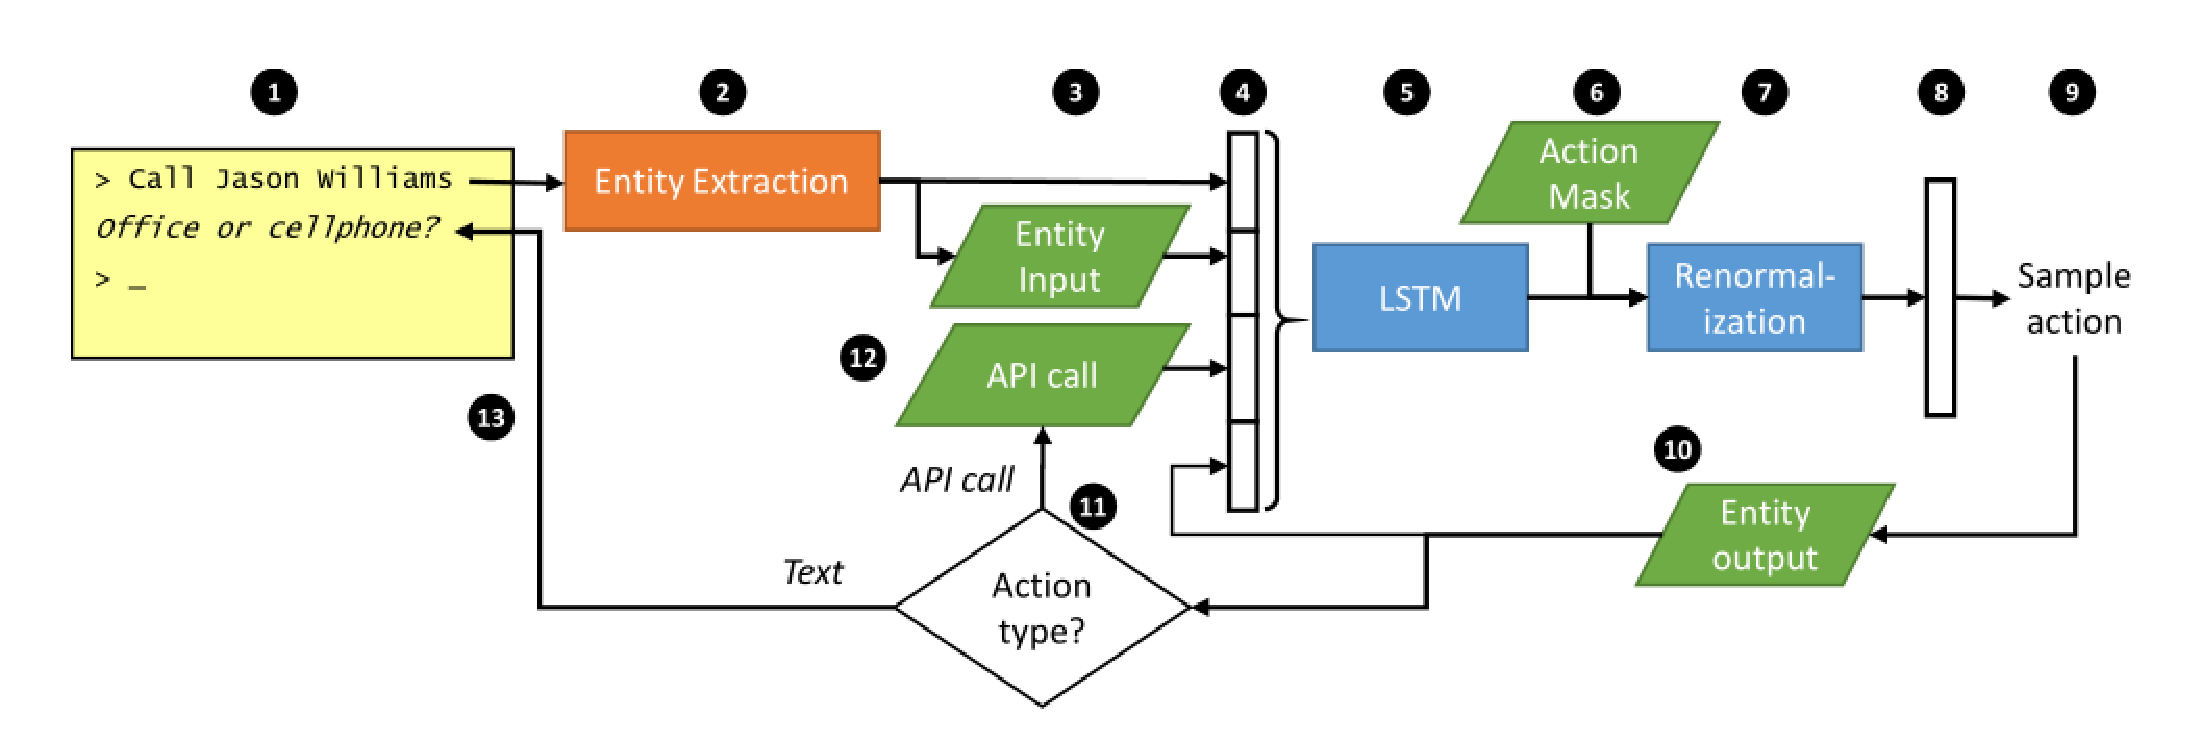
\includegraphics[width=\linewidth]{Williams2016End01}\\
  \caption{Operational loop of a dialogue system}\label{fig:Williams2016End01}
\end{figure}

The operational cycle has 13 steps: (1) The system receives user input; (2) The entities mentioned in user input are identified; (3) The extracted entities are resolved into ground entities corresponding to one or more rows in a database; (4) A feature vector is constructed from four sources; (5) LSTM takes the feature vector, update its hidden states, and outputs a distribution over all template actions; (6) Domain-specific software provides an action mask indicating actions that are not allowed at the current time; (7, 8) The task mask is combined with the distribution in step five into a new distribution; (9) An action is chosen from the new distribution; (10) The selected template action is instantiated with the entities in step three; (11, 12, 13) Depending on the action type, the system either invokes the corresponding API call or render the response text to users. 